\section{区域积分}
\label{sec:multivariable-region-integration}

一块不均匀的金属薄片占据平面区域$D$，在点$(x,y)$附近每单位面积的质量为$\rho(x,y)$。
把$D$切成许多小块，每块的质量约等于块内某一点的密度乘这块的面积；把所有小块的质量相加，就得到总质量的近似值，小块切得越细，近似越准确。
空间物体的质量、带电体的总电荷也按同样方式累计，只是面积换成体积，面密度换成体密度或电荷密度。
这类问题中的被积函数都是多元标量函数$f:D\subseteq\mathbb R^d\to\mathbb R$：输入是一个位置的$d$个坐标，输出是该位置上一个待累计的数。

同一个积分还有两种常用读法。
若$f\geq0$定义在平面区域$D$上，积分等于以$D$为底、以$f$的图像为顶的立体的体积，这是一元积分“曲线下方面积”在高一维的对应。
把积分除以$D$的面积，所得的数是$f$在$D$上的平均值，例如一个地区的平均降雨量或一块薄板的平均温度。

第~\ref{sec:analysis-measurability-integration}节在实轴上用长度给小块赋权，再由简单函数逼近和绝对可积要求建立了勒贝格积分。
推广到$\mathbb R^d$时只需更换两样东西：小块的大小改用$d$维体积来度量，函数的输入改为$\mathbb R^d$中的点。
简单函数逼近、单调收敛和支配收敛的论证只用到“分层、相加、取极限”，不依赖输入有几个坐标，可以原样沿用。

定义建立以后，还要回答计算上的三个问题。
第一，能否先算每一条切片上的累计，再把各切片的结果累加，也就是把区域积分拆成逐个坐标的一元积分？答案取决于非负性或绝对可积性，它们保证两种累计次序给出同一个区域积分。
第二，圆盘、球体等区域在直角坐标下边界复杂，能否改用极坐标、球坐标描述？换坐标会放大或缩小每个小块的体积，需要用Jacobian行列式校正。
第三，被积函数依赖一个参数时，积分值怎样随参数变化，能否在积分号下求导？
本节先建立多维测度与区域积分，再依次讨论这三个问题。切片与坐标计算的更多例题可参考\scite{math-openstax-calculus3}。

\subsection{多维测度与乘积测度}
\label{sec:comb-multidimensional-product-measure}

区域积分首先要回答“一块区域有多大”。
实轴上的长度已经由勒贝格测度给出；平面上的面积、空间中的体积也需要同样精确的定义，否则无法给边界弯曲、带有无穷多个小洞或形状不规则的区域赋予大小。
本小节先把第~\ref{sec:comb-set-measurement}节的区间覆盖构造搬到$\mathbb R^d$，再说明把$\mathbb R^d$拆成$\mathbb R^p\times\mathbb R^q$（$d=p+q$）时，$d$维体积怎样由$p$维与$q$维的体积相乘得到。
后一点是第~\ref{sec:multivariable-iterated-integrals}节累次积分成立的测度基础。

\subsubsection{多维勒贝格测度}

\paragraph{坐标盒}

实轴上的构造从区间出发，因为区间的长度不需要另行定义。
$\mathbb R^d$中与区间对应的对象是各坐标方向上区间的笛卡尔积，称为坐标盒，例如
\[
 Q=\prod_{i=1}^d(a_i,b_i),\qquad a_i<b_i.
\]
平面上的坐标盒是各边平行于坐标轴的长方形，空间中的坐标盒是长方体。
坐标盒的体积规定为各边长之积$\operatorname{vol}(Q)=\prod_i(b_i-a_i)$，例如$(0,2)\times(0,3)$的面积为$6$。
这条规定推广了长方形面积公式，也与有限集合的计数规则$|A\times B|=|A||B|$一致：一个方向排$m$个单位格、另一个方向排$n$个单位格时，共有$mn$个单位格。
闭盒、半开盒与同端点开盒的体积相同；某一边长为零的退化盒，例如平面上的一条线段，体积为零。

\paragraph{多维勒贝格测度}

一维外测度用可数个区间覆盖集合，再取覆盖总长度的下确界。
把区间换成开坐标盒、把长度换成体积，就得到$\mathbb R^d$上的外测度
\[
 m_d^*(E)=\inf_{\substack{E\subseteq\bigcup_{n=1}^{\infty}Q_n\\
 Q_n\text{为开坐标盒}}}\sum_{n=1}^{\infty}\operatorname{vol}(Q_n),
\]
其中下确界取遍$E$的所有可数开盒覆盖。
直观上，这是用盒子从外侧包住$E$，看至少需要多少总体积。

按这个定义，线段和可数点集的面积都是零。
线段$[0,1]\times\{0\}$能被一个开盒$(-\varepsilon,1+\varepsilon)\times(-\varepsilon,\varepsilon)$覆盖，这个盒的面积$2\varepsilon(1+2\varepsilon)$可以任意小，所以线段的二维外测度为零：线段有长度，却没有面积。
把$\mathbb Q^2$的点排成一列，第$k$个点放进面积为$\varepsilon2^{-k}$的小盒，这些小盒的总面积不超过$\varepsilon$，因此$\mathbb Q^2$的二维外测度也为零，论证与实轴上可数集零测相同。

可测集仍沿用定义~\ref{def:analysis-lebesgue-measurable-set}的分割要求：若集合$A\subseteq\mathbb R^d$对每个测试集合$E\subseteq\mathbb R^d$满足
$m_d^*(E)=m_d^*(E\cap A)+m_d^*(E\setminus A)$，就称$A$为$d$维勒贝格可测集。
一维情形中关于外测度的可数次可加性、可测集族构成$\sigma$代数、测度的可数可加性以及零测集子集可测的论证，只用到覆盖、取下确界和分割这几种操作，没有用到区间只有一个方向，所以把区间换成盒以后可以逐步照搬。
于是$d$维勒贝格可测集组成$\sigma$代数$\mathcal L(\mathbb R^d)$；把$m_d^*$限制在$\mathcal L(\mathbb R^d)$上，得到$d$维勒贝格测度$m_d$，其中$m_1$就是第~\ref{sec:comb-set-measurement}节的$m$。
$m_d$是完备的，即零测集的子集都可测。
需要另作核对的只有$m_d(Q)=\operatorname{vol}(Q)$，即可数个盒的覆盖不会把一个盒的体积算小；它对应一维中“区间的外测度等于其长度”的论证，这里不再重复。

常用的集合都在这个可测范围内。
坐标半空间$\{\bm x:x_i\leq t\}$的可测性与一维半直线相同：把每个覆盖盒沿超平面$x_i=t$切成两块，两块的体积之和仍是原盒的体积；坐标盒由这类半空间经取补集和可数次交、并得到，因而也可测。
每个欧氏开集又都是其中有理端点开盒的可数并：对开集中的每一点，先取一个包含该点且完全落在开集内的开盒，再把端点向内调整为有理数，使盒仍包含该点；有理端点的盒只有可数个。
因此$\mathcal L(\mathbb R^d)$包含全部开集，从而包含由全部开集（等价地，由全部开盒）生成的Borel $\sigma$代数$\mathcal B(\mathbb R^d)$；由于$m_d$完备，勒贝格范围还包含Borel零测集的全部子集。

\paragraph{平移与伸缩}

把集合$E$平移一个向量$\bm a$，每个覆盖盒也随之平移，盒的边长不变，所以$m_d(E+\bm a)=m_d(E)$。
把集合按比例$c>0$伸缩为$cE=\{c\bm x:\bm x\in E\}$时，每个覆盖盒的每条边都乘$c$，体积乘$c^d$，而$E$的覆盖与$cE$的覆盖一一对应，因此
\[
 m_d(cE)=c^dm_d(E).
\]
这正是“长度按$c$倍、面积按$c^2$倍、体积按$c^3$倍变化”的精确形式。
例如平面圆环$\{1\leq\lVert\bm x\rVert_2<2\}$放大$2^k$倍后得到$\{2^k\leq\lVert\bm x\rVert_2<2^{k+1}\}$，面积变为原来的$4^k$倍；示例~\ref{ex:region-power-function-threshold}判别幂函数的可积性时会用到这个事实。
一般线性映射对体积的放大倍数是行列式的绝对值，留到第~\ref{sec:multivariable-change-variables}节讨论。

\subsubsection{乘积测度}

累次积分要把$\mathbb R^d$看成$\mathbb R^p\times\mathbb R^q$，先在$\mathbb R^q$方向累计，再在$\mathbb R^p$方向累计。
为此需要知道$d$维体积与$p$维、$q$维体积之间的关系。
对坐标盒，答案已经包含在定义里：$d$条边长之积等于前$p$条边长之积乘后$q$条边长之积。
还需要确认两件事：对一般的Borel集合$A\subseteq\mathbb R^p$与$B\subseteq\mathbb R^q$，乘积集合$A\times B$（下文称为矩形）的体积是否仍为$m_p(A)m_q(B)$；只规定矩形的体积，能否唯一确定其余集合的$d$维体积。

\paragraph{矩形赋值的乘法规则}

矩形上的乘法规则可以先在只有有限个格子的情形中看清。
\begin{example}[有限网格上的乘积权重]
\label{ex:region-finite-product-weights}
横向分为两列，权重（可以理解为两段的长度或两组点的总质量）分别为$1,2$；纵向分为两行，权重分别为$3,4$。
规定每个格子的联合权重等于所在列、行权重之积，四个格子的权重就是$1\cdot3=3$、$2\cdot3=6$、$1\cdot4=4$、$2\cdot4=8$。
逐格相加得到总量
\[
 3+6+4+8=21=(1+2)(3+4),
\]
右侧先把两侧权重各自相加再相乘，两侧相等正是有限分配律。
先求每一行的总量$3+6=9$、$4+8=12$再相加，或先求每一列的总量$3+4=7$、$6+8=14$再相加，也都得到$21$。
\end{example}

逐格、逐行、逐列三种求和次序给出同一个总量，这就是累次积分在有限情形中的样子。
图~\ref{fig:analysis-process-product-measure-grid}把列宽和行高分别按两侧权重画成比例，格子面积因而等于乘积权重。
乘法规则只描述一种特定的联合赋权方式，一般的二元分布不必由两侧权重相乘得到。

\begin{figure}[!htbp]
 \centering
 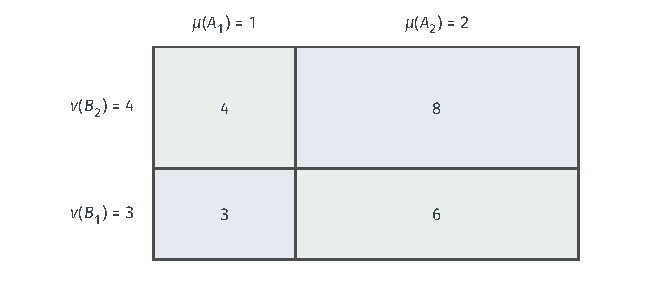
\includegraphics[width=112mm]{figures/01-mathematical-preliminaries-upper/00-shared/tikz/chapter3-concept-processes/product-measure-grid.pdf}
 \caption{两列的权重分别为$1,2$（图中记为$\mu(A_1),\mu(A_2)$），两行的权重分别为$3,4$（记为$\nu(B_1),\nu(B_2)$）。四个格子的乘积权重为$3,6,4,8$，总量$21=(1+2)(3+4)$。列宽与行高按各自权重成比例，因此格子面积也按乘积成比例。这只是乘积赋权的有限示例，并非任意二维分布都满足的关系。}
 \label{fig:analysis-process-product-measure-grid}
\end{figure}

\paragraph{乘积$\sigma$代数}

矩形适合规定基本赋值，但矩形的并或补一般不再是矩形，例如两个长方形拼成的L形区域就不是矩形，因此不能只把矩形本身当作全部可测集合。
设$A\in\mathcal B(\mathbb R^p)$、$B\in\mathcal B(\mathbb R^q)$，称$A\times B$为Borel矩形。
包含全部Borel矩形的最小$\sigma$代数称为乘积$\sigma$代数，记为$\mathcal B(\mathbb R^p)\otimes\mathcal B(\mathbb R^q)$。
它和直接在$\mathbb R^{p+q}$中由开盒生成的Borel范围是同一个集合族：
\begin{equation}
 \mathcal B(\mathbb R^p)\otimes\mathcal B(\mathbb R^q)=\mathcal B(\mathbb R^{p+q}).
 \label{eq:comb-borel-product-structure}
\end{equation}

先证右侧包含于左侧。$\mathbb R^{p+q}$中的每个开盒都是$\mathbb R^p$中一个开盒与$\mathbb R^q$中一个开盒的乘积，因而是Borel矩形；每个开集又是可数个开盒的并，所以全部开集都在左侧，左侧作为$\sigma$代数就包含它们生成的$\mathcal B(\mathbb R^{p+q})$。

再证左侧包含于右侧，只需说明每个Borel矩形都是$\mathbb R^{p+q}$中的Borel集合。
考虑所有满足$A\times\mathbb R^q\in\mathcal B(\mathbb R^{p+q})$的集合$A\subseteq\mathbb R^p$。
开盒$A$使$A\times\mathbb R^q$成为开集，所以开盒都满足要求；又因为$(\mathbb R^p\setminus A)\times\mathbb R^q$是$A\times\mathbb R^q$的补集、$\bigl(\bigcup_nA_n\bigr)\times\mathbb R^q=\bigcup_n(A_n\times\mathbb R^q)$，满足要求的集合对补集和可数并封闭。
这些集合因而构成一个包含开盒的$\sigma$代数，从而包含全部$\mathcal B(\mathbb R^p)$。
同理$\mathbb R^p\times B$对每个$B\in\mathcal B(\mathbb R^q)$都是Borel集合，于是
$A\times B=(A\times\mathbb R^q)\cap(\mathbb R^p\times B)$属于$\mathcal B(\mathbb R^{p+q})$。
左侧的生成集合都在右侧，所以左侧包含于右侧。

\paragraph{乘积测度}

有了可测范围，还要为其中每个集合赋予联合的大小。对Borel矩形，所需规则就是把两个方向的测度相乘。

\begin{definition}[乘积测度]
\label{def:analysis-product-measure}
设$p,q\geq1$。在$\mathcal B(\mathbb R^p)\otimes\mathcal B(\mathbb R^q)$上，若一个测度对所有$A\in\mathcal B(\mathbb R^p)$、$B\in\mathcal B(\mathbb R^q)$满足
\begin{equation}
 (m_p\otimes m_q)(A\times B)=m_p(A)m_q(B),
 \label{eq:comb-product-measure-rectangle}
\end{equation}
就称它为$m_p$与$m_q$的\term{乘积测度}（product measure），记为$m_p\otimes m_q$，其中约定$0\cdot\infty=0$。
\end{definition}

约定$0\cdot\infty=0$有直观依据：平面上的直线$\mathbb R\times\{0\}$在横向长度无穷、纵向长度为零，它应当没有面积。
定义只规定了矩形应有的测度，还要确认这个规定能够一致地扩展到整个乘积$\sigma$代数，并且扩展只有一种。

\begin{theorem}[乘积测度的存在唯一性]
在$\mathcal B(\mathbb R^p)\otimes\mathcal B(\mathbb R^q)$上恰有一个测度满足式~\eqref{eq:comb-product-measure-rectangle}，它就是$m_{p+q}$在$\mathcal B(\mathbb R^{p+q})$上的限制。
\end{theorem}

存在性由$m_{p+q}$本身提供：对坐标盒，矩形规则就是体积的定义；从盒推进到一般Borel矩形，要利用两侧Borel集合都能被可数个盒从外侧逼近，这一步引用测度论教材\scite{math-folland1999real}。
唯一性的论证依赖两点：两个矩形的交仍是矩形；$\mathbb R^{p+q}$能被可数个有限体积的盒$(-n,n)^{p+q}$逐步填满。
两个测度若在全部矩形上取值相同，先在每个有限体积的盒内比较，再令$n\to\infty$，就能推出它们在整个乘积$\sigma$代数上相同，完整论证见同一教材。
两个一般测度空间也可以按同样的矩形规则作乘积，那时“能被可数个有限测度部分填满”成为必须单独检查的条件；一般的构造与条件见第~\ref{chap:measure-spaces}章。

\paragraph{欧氏乘积与完备化}

上面的乘积测度只定义在Borel范围上，而区域积分使用的是更大的勒贝格范围$\mathcal L(\mathbb R^{p+q})$。
两者之间相差的只是零测集的子集：每个勒贝格可测集都能写成一个Borel集合与某个Borel零测集的子集之并\scite{math-folland1999real}。
把这些零测集的子集也补进可测范围，称为完备化；$m_{p+q}$在$\mathcal L(\mathbb R^{p+q})$上正是$m_p\otimes m_q$的完备化。

完备化不能靠先把两个因子完备化来代替：即使两个因子都取完备的勒贝格测度，它们的乘积$\sigma$代数也未必完备。
\begin{example}[勒贝格因子的乘积$\sigma$代数不完备]
\label{ex:region-product-sigma-algebra-incomplete}
取$p=q=1$，考虑由全部乘积$A\times B$（$A,B\in\mathcal L(\mathbb R)$）生成的乘积$\sigma$代数$\mathcal L(\mathbb R)\otimes\mathcal L(\mathbb R)$。

先说明其中每个集合$E$在每个$x$处的截面$E_x=\{y:(x,y)\in E\}$都勒贝格可测。
截面都可测的集合组成的族包含全部乘积$A\times B$，因为$(A\times B)_x$是$B$或$\varnothing$。取截面与取补集、可数并可以交换次序：$(\mathbb R^2\setminus E)_x=\mathbb R\setminus E_x$，$\bigl(\bigcup_nE_n\bigr)_x=\bigcup_n(E_n)_x$；所以这个族是$\sigma$代数，从而包含整个乘积$\sigma$代数。

再取一个勒贝格不可测集$S\subseteq\mathbb R$（第~\ref{sec:comb-set-measurement}节指出这类集合存在），令$E=\{0\}\times S$。
$E$包含在直线$\{0\}\times\mathbb R$中。这条直线是乘积$\{0\}\times\mathbb R$，乘积测度给它的值为$m(\{0\})m(\mathbb R)=0\cdot\infty=0$，所以$E$是乘积测度下零测集的子集；在完备的勒贝格范围$\mathcal L(\mathbb R^2)$中，$E$可测且零测。
但$E$在$x=0$处的截面是不可测集$S$，所以$E$不属于乘积$\sigma$代数。
\end{example}

因此下面陈述累次积分时，要分清函数对Borel范围可测，还是只对勒贝格范围可测；后者的结论需要附加“几乎处处”。

\subsection{区域积分的定义与可积性}
\label{sec:multivariable-riemann-lebesgue}

测度确定区域有多大，被积函数确定各位置贡献多少。
现在把一元可测函数与勒贝格积分的定义搬到$\mathbb R^d$上：改变的是输入空间和所用的测度，积分的构造步骤不变。

\subsubsection{多元可测函数}

累计函数值时，要把输入按函数值分层，例如取值在$[u,v)$之间的位置组成一层，这一层的贡献约为函数值乘该层的体积。
只有每一层都能测量，这种累计才有意义。
与一元情形一样，只需检查所有阈值集合$\{f>a\}$，因为$\{f\geq u\}=\bigcap_n\{f>u-1/n\}$、$\{u\leq f<v\}=\{f\geq u\}\setminus\{f\geq v\}$等集合都能由阈值集合经可数次集合运算得到。
\begin{definition}[多元可测函数]
设$D\in\mathcal L(\mathbb R^d)$。函数$f:D\to\overline{\mathbb R}$称为勒贝格可测函数，是指对每个$a\in\mathbb R$，集合
\[
 \{\bm x\in D:f(\bm x)>a\}
\]
都属于$\mathcal L(\mathbb R^d)$。若这些集合都属于$\mathcal B(\mathbb R^d)$，则称$f$为Borel可测函数。
\end{definition}

连续函数都可测：若$f$在$D$上连续，阈值集合$\{f>a\}$是开区间$(a,\infty)$的原像，因而相对于$D$开，可写为$D$与某个欧氏开集之交；$D$与开集都可测，所以阈值集合可测。
连续性只是可测性的充分条件：$\mathbb I_{\mathbb Q^d}$处处不连续，却是可测函数，因为它的阈值集合在$a<0$、$0\leq a<1$、$a\geq1$时分别是全空间、$\mathbb Q^d$和$\varnothing$，而可数集$\mathbb Q^d$零测，因而可测。

第~\ref{sec:analysis-measurable-functions}节关于和、积、绝对值、最大最小值以及逐点极限保持可测性的论证只用到阈值集合的可数运算，在$\mathbb R^d$上照样成立。
例如分段给出的函数$f=g\mathbb I_{D_1}+h\mathbb I_{D_2}$，只要$g,h$在$\mathbb R^d$上连续、$D_1,D_2$可测，就是可测函数。
向量值函数的积分按分量进行，每个分量都是本节讨论的标量函数；例如质心的每个坐标都是一个标量区域积分与总质量之比。

\subsubsection{区域积分的定义}

\paragraph{非负标量函数的积分}

先累计非负贡献，就不会遇到正负无穷相消。
可测简单函数在每个可测小块上取常值，其积分等于各块的常值乘该块测度再求和；一般非负函数仍由下方的简单函数逼近。
\begin{definition}[区域上非负可测函数的积分]
设$D\in\mathcal L(\mathbb R^d)$，$f:D\to[0,\infty]$可测。定义
\[
 \int_D f\,\mathrm dm_d
 =\sup_{\substack{0\leq s\leq f\\s\text{为可测简单函数}}}
 \int_D s\,\mathrm dm_d.
\]
若$s=\sum_{j=1}^n c_j\mathbb I_{E_j}$，其中$E_j\subseteq D$可测、两两不交且$c_j\geq0$，则$\int_Ds\,\mathrm dm_d=\sum_jc_jm_d(E_j)$，约定$0\cdot\infty=0$。
\end{definition}

把$f$看成薄片的面密度，就能读出这个定义的含义。
满足$0\leq s\leq f$的简单函数把区域分成有限块，并在每块上用一个不超过真实密度的常数代替密度，所以$\int_Ds$是总质量的一个偏小估计；对所有这样的估计取上确界，就得到总质量。

也可以从体积来读：$c_j\mathbb I_{E_j}$对应以$E_j$为底、高为$c_j$的柱体$E_j\times[0,c_j)$，由乘积测度的矩形规则，它的$(d+1)$维体积就是$c_jm_d(E_j)$。
于是$\int_Ds$是排在$f$的图像下方的一组柱体的总体积，上确界则是图像下方整个区域的体积；第~\ref{sec:multivariable-iterated-integrals}节会用Tonelli定理把这个读法写成等式。

这个积分可以取$+\infty$，例如$f\equiv1$在整个平面上的积分是平面的面积$+\infty$。
在全空间上把$f$作零延拓，就有
$\int_Df\,\mathrm dm_d=\int_{\mathbb R^d}f\mathbb I_D\,\mathrm dm_d$，其中$f\mathbb I_D$在$D$内等于$f$、在$D$外取零；以后在区域上积分，都可以看成对零延拓后的函数在全空间上积分。
区域不必是矩形，定义也不要求它的边界零测；这与黎曼积分先用矩形网格逼近区域的做法不同。

\paragraph{有符号标量函数的积分}

函数可以取正负值时，例如带电薄片上既有正电荷也有负电荷，应先分别累计正负贡献：$f^+=\max\{f,0\}$给出正电荷的密度，$f^-=\max\{-f,0\}$给出负电荷的密度，净电荷是两者总量之差。
与一元情形相同，为了让这个差是一个普通的有限数，要求绝对值的总贡献有限。
\begin{definition}[区域上可测函数的积分]
设$D\in\mathcal L(\mathbb R^d)$，$f:D\to\overline{\mathbb R}$可测。若
\begin{equation}
 \int_D|f|\,\mathrm dm_d<\infty,
 \label{eq:multivariable-lebesgue-integrability}
\end{equation}
称$f$在$D$上勒贝格可积，并定义
\[
 \int_Df\,\mathrm dm_d=\int_Df^+\,\mathrm dm_d-\int_Df^-\,\mathrm dm_d.
\]
\end{definition}

由于$|f|=f^++f^-$，条件~\eqref{eq:multivariable-lebesgue-integrability}同时保证正负两部分的积分都有限，相减不会出现$\infty-\infty$。
这个条件不成立时，至少有一部分积分为无穷；若两部分都为无穷，两者之差没有意义，也就不能用相减定义勒贝格积分。

条件~\eqref{eq:multivariable-lebesgue-integrability}还保证$f$几乎处处取有限值。
集合$N=\{|f|=\infty\}$对每个$M>0$满足$M\mathbb I_N\leq|f|$，所以$Mm_d(N)\leq\int_D|f|$对所有$M$成立，只能$m_d(N)=0$；在$N$上把无穷值改成零，不改变积分。

与黎曼积分相比，这一定义不要求函数在细小的网格块上接近常数。
例如$\mathbb I_{\mathbb Q^d}$在单位立方体上不黎曼可积：每个小盒中都既有有理点又有无理点，上和恒为$1$而下和恒为$0$；但它的勒贝格积分为零，因为可数集的$d$维测度为零。

\paragraph{二重积分与多重积分}

二维时把上述积分写为
\[
 \iint_Df(x,y)\,\mathrm dx\,\mathrm dy=\int_Df\,\mathrm dm_2;
\]
三维中常记为$\iiint_Df\,\mathrm dV$；$d$维时统一写作
\[
 \int_Df(\bm x)\,\mathrm d\bm x=\int_Df\,\mathrm dm_d.
\]
“二重”或“多重”表示输入维数，并不表示已经选择了逐坐标的计算次序。
例如$f\equiv3$、$D=[0,1]\times[0,2]$时，积分为$3m_2(D)=6$：密度处处为$3$、面积为$2$的薄片，总质量为$6$。

当$0<m_d(D)<\infty$且$f$可积时，
\[
 \frac{1}{m_d(D)}\int_Df\,\mathrm dm_d
\]
称为$f$在$D$上的平均值。
它是一个常数，用它代替$f$铺满整个$D$，总累计不变。上例的平均值为$3$。

\subsubsection{可积性的判别}

按定义，可测函数$f$在$D$上可积，意思是非负积分$\int_D|f|\,\mathrm dm_d$有限。
这个非负积分总有定义，只是可能等于$+\infty$；判别可积性因此只需回答一个问题：$|f|$在$D$上的总累计是有限还是无穷。
直接从上确界定义计算这个量往往不现实，下面三种做法都用更容易得到的量来估计它：用函数的上界乘区域的测度；用一列测度有限的递增子区域逼近$D$，看这些子区域上的累计是否有共同上界；与一个已知是否可积的函数逐点比较。

若$f$有界且$D$的测度有限，第一种做法立即给出有限上界。
由此可见，累计变为无穷只能是因为$f$无界（例如在某些位置附近无界），或者$D$的测度无穷；后两种做法正是为这两种情形准备的。

\paragraph{有界函数且有界区域}

设区域$D$有界，从而$m_d(D)<\infty$（更一般地，只要$m_d(D)<\infty$即可），$f$可测且$|f|\leq M<\infty$几乎处处成立。
这时$|f|\leq M\mathbb I_D$几乎处处成立，由非负积分的单调性，
\[
 \int_D|f|\,\mathrm dm_d\leq M m_d(D)<\infty.
\]
物理上，总质量不超过最大密度乘面积。
由定理~\ref{thm:multivariable-extreme-value}，闭有界集上的连续函数有界，所以闭有界区域上的连续函数可积。

这一判别只用到有界性，不要求函数能连续地延伸到区域的边界。
\begin{example}[开正方形上剧烈振荡的有界函数可积]
\label{ex:region-bounded-oscillation}
在开正方形$(0,1)^2$上令$f(x,y)=\sin\bigl(1/(xy)\bigr)$。
$f$在开正方形上连续，因而可测。
它不能连续延拓到闭正方形：固定$x=t\in(0,1)$，令$y\downarrow0$，则$1/(ty)\to+\infty$，$f(t,y)$在$-1$与$1$之间无穷次振荡，没有极限。
所以闭有界集上的极值定理不能直接使用。
但$|f|\leq1$且$m_2\bigl((0,1)^2\bigr)=1$，由上面的估计，
\[
 \int_{(0,1)^2}|f|\,\mathrm dm_2\leq1,
\]
所以$f$在$(0,1)^2$上可积。
\end{example}

这个判别不适用于两类情形：函数无界，或区域的测度无穷。
在这两类情形中，可积与不可积都可能发生。
无界函数仍可能可积，示例~\ref{ex:region-power-function-threshold}将说明$\lVert\bm x\rVert_2^{-1}$在平面单位圆盘上可积；无限测度区域上的有界函数则未必可积，例如$f\equiv1$在整个平面上积分为无穷。
判断这两类情形需要更细的估计。

\paragraph{无界函数或无限区域}

处理无界函数或无限区域时，可以先避开麻烦的位置。
取一列递增的可测集合$D_1\subseteq D_2\subseteq\cdots$，使$\bigcup_nD_n=D$，并让每个$D_n$避开函数无界的位置、只占有限测度；例如函数只在原点附近无界时，可取$D_n=D\cap\{1/n\leq\lVert\bm x\rVert_2\leq n\}$。
这时每个$\int_{D_n}|f|$通常可以用有界函数在有限测度区域上的估计确认有限。
由于$0\leq|f|\mathbb I_{D_n}\uparrow|f|\mathbb I_D$，单调收敛定理（定理~\ref{thm:analysis-monotone-convergence}）给出
\[
 \int_D|f|\,\mathrm dm_d
 =\lim_{n\to\infty}\int_{D_n}|f|\,\mathrm dm_d
 =\sup_n\int_{D_n}|f|\,\mathrm dm_d.
\]
因此$f$在$D$上可积，当且仅当截断累计$\int_{D_n}|f|$有一个与$n$无关的有限上界。
这就是定理~\ref{thm:analysis-improper-nonnegative-criterion}在$\mathbb R^d$中的形式，证明只用单调收敛，不依赖维数。
只知道每个截断累计分别有限还不够，必须检查它们是否共同有界。

截断累计也可以改写成级数。
把区域拆成两两不交的“壳层”$A_k=D_k\setminus D_{k-1}$（$D_0=\varnothing$），由积分的区域可加性（定理~\ref{thm:analysis-integral-set-additivity}），
$\int_D|f|=\sum_k\int_{A_k}|f|$，可积性就化为一个非负级数是否收敛。

只依赖半径的函数适合用壳层估计。
下面按半径成倍增长划分壳层，判别平面幂函数在原点附近和远处的可积性。
\begin{example}[平面幂函数$\lVert\bm x\rVert_2^{-p}$的可积阈值]
\label{ex:region-power-function-threshold}
设$p>0$，$f(\bm x)=\lVert\bm x\rVert_2^{-p}$，$\bm x\in\mathbb R^2\setminus\{\bm 0\}$。按半径成倍增长的圆环
\[
 A_k=\{\bm x\in\mathbb R^2:2^k\leq\lVert\bm x\rVert_2<2^{k+1}\},\qquad k\in\mathbb Z
\]
把$\mathbb R^2\setminus\{\bm 0\}$分成两两不交的壳层。

记$\alpha=m_2(A_0)$。它是一个有限正数：$A_0$含有小盒，又含于盒$(-2,2)^2$。
由伸缩性质，$A_k=2^kA_0$，所以$m_2(A_k)=4^k\alpha$。
在$A_k$上$2^{-(k+1)p}<\lVert\bm x\rVert_2^{-p}\leq2^{-kp}$，乘以$m_2(A_k)$得到
\[
 2^{-p}\alpha\,2^{k(2-p)}\leq\int_{A_k}\lVert\bm x\rVert_2^{-p}\,\mathrm d\bm x\leq\alpha\,2^{k(2-p)}.
\]

单位圆外由$k=0,1,2,\ldots$的壳层组成，各壳层的贡献与公比为$2^{2-p}$的几何级数同阶，累计有限当且仅当$p>2$。
单位圆内（去掉原点）由$k=-1,-2,\ldots$的壳层组成；令$j=-k$，各壳层的贡献与$2^{j(p-2)}$同阶，累计有限当且仅当$p<2$。
因此$\lVert\bm x\rVert_2^{-p}$在单位圆盘上可积当且仅当$p<2$，在单位圆外可积当且仅当$p>2$；$p=2$时两侧都不可积，在整个平面上则对任何$p>0$都不可积。
\end{example}

在$\mathbb R^d$中把面积因子$4^k$换成$2^{kd}$，同样的计算给出阈值$d$；$d=1$就是第~\ref{sec:analysis-improper-integrals}节的阈值$1$。
这个阈值比较的是两种速度：靠近原点时，函数按$r^{-p}$增大，而半径约为$r$的壳层的体积按$r^d$缩小；远离原点时，函数按$r^{-p}$减小，壳层的体积按$r^d$增大。
第~\ref{sec:multivariable-change-variables}节将用极坐标直接计算圆环上的积分，验证这里的结论（示例~\ref{ex:region-polar-power-check}）。

确认可积以后，截断积分还能用来计算有符号积分。
由$|f\mathbb I_{D_n}|\leq|f|$，支配收敛定理（定理~\ref{thm:analysis-dominated-convergence}）给出$\int_{D_n}f\to\int_Df$，误差不超过$\int_{D\setminus D_n}|f|$，所以无论选哪一列递增区域，都得到同一个值。

缺少绝对可积性时，截断极限可能依赖区域的选法。
\begin{example}[截断极限依赖截断方式]
\label{ex:region-truncation-dependence}
在平面上令$f(x,y)=1$（$x>0$），$f(x,y)=-1$（$x\leq0$）。
取正方形$D_n=(-n,n)^2$时，右半部分与左半部分的面积都是$2n^2$，正负贡献恰好抵消，每个$\int_{D_n}f=0$。
取偏向右侧的长方形$D_n'=(-n,2n)\times(-n,n)$时，右侧部分面积为$4n^2$，左侧部分面积为$2n^2$，所以$\int_{D_n'}f=2n^2\to+\infty$。
两列截断都递增地填满整个平面，极限却分别是$0$和$+\infty$。
\end{example}

例中$\int|f|=+\infty$，两种截断的不同极限都不能当作$f$的积分。
截断只能用来计算已经确认绝对可积的函数的积分。

\paragraph{比较判别：可积上界与不可积下界}

有了一族可积性已知的函数，就可以把新函数与它们逐点比较，而不必每次重新做壳层计算。
比较有两个方向，都来自非负积分的单调性：
\begin{itemize}
 \item 若存在非负可积函数$H$，使$|f|\leq H$在$D$上几乎处处成立，则$\int_D|f|\leq\int_DH<\infty$，$f$可积；
 \item 若存在非负可测函数$g$，使$|f|\geq g$在$D$上几乎处处成立且$\int_Dg=+\infty$，则$\int_D|f|=+\infty$，$f$不可积。
\end{itemize}
比较只需在可能出问题的位置进行：先用区域可加性把$D$拆成函数有界且测度有限的部分和“原点附近”“远处”等部分，前者用有界判别，其余部分再与幂函数比较。

远处的比较看函数衰减得有多快。
\begin{example}[远处与$r^{-3}$和$r^{-2}$比较]
\label{ex:region-comparison-at-infinity}
记$r=\lVert\bm x\rVert_2$，其中$\bm x=(x,y)$。

函数$f(x,y)=\cos(xy)/(1+x^2+y^2)^{3/2}$在整个平面上可积。
在单位圆盘内$|f|\leq1$，用有界判别；在单位圆外$|f|\leq(1+r^2)^{-3/2}\leq r^{-3}$，而由示例~\ref{ex:region-power-function-threshold}，$p=3>2$的幂函数在圆外可积。

函数$g(x,y)=1/(1+x^2+y^2)$在整个平面上不可积。
在单位圆外$1+r^2\leq2r^2$，所以$g\geq r^{-2}/2$，而$p=2$的幂函数在圆外累计无穷。
\end{example}

一元的$1/(1+x^2)$在实轴上可积，二元的类似函数却不可积。
原因在于远处可用的范围增长得更快：半径为$R$的圆盘面积按$R^2$增长，而区间$[-R,R]$的长度只按$R$增长。

原点附近的比较同样只看奇点处的增长速度。
\begin{example}[原点附近的对数奇点与平方倒数奇点]
\label{ex:region-comparison-near-origin}
仍记$r=\lVert\bm x\rVert_2$，在单位圆盘$\{r\leq1\}$上考察两个在原点附近无界的函数。

$\log(x^2+y^2)=2\log r$在$r\downarrow0$时趋于$-\infty$。
函数$t\mapsto t|\log t|$在$(0,1)$上的最大值为$1/e$，在$t=1/e$处取到，所以$0<r<1$时
\[
 |\log r^2|=2|\log r|\leq\frac2e\,r^{-1}.
\]
与$p=1<2$的幂函数比较，可知$\log(x^2+y^2)$在单位圆盘上可积。

$(x^2+2y^2)^{-1}$满足$x^2+2y^2\leq2(x^2+y^2)=2r^2$，所以$(x^2+2y^2)^{-1}\geq r^{-2}/2$。
与$p=2$的幂函数比较，可知它在单位圆盘上不可积。
\end{example}

找不到合适的比较函数时，还可以用第~\ref{sec:multivariable-iterated-integrals}节的Tonelli定理把$\int_D|f|$化为累次积分直接计算，再判断它是否有限。

\subsection{区域积分的基本性质}

多维区域积分仍是按第~\ref{sec:analysis-measurability-integration}节方式构造的勒贝格积分，只是测度换成了$m_d$。
那里的单调收敛定理、Fatou引理、支配收敛定理以及下面各条积分性质，证明都只用到简单函数逼近、测度的可数可加性和这些结论之间的推导，不依赖输入只有一个坐标，因此在$\mathbb R^d$上可以直接使用。
下面固定可测区域$D$，各有符号公式均要求所列函数在相应区域上绝对可积，微元统一写为$\mathrm dm_d$。

\paragraph{加法}

若$f,g$在$D$上可积，则$f+g$也可积，且
\[
 \int_D(f+g)\,\mathrm dm_d=\int_Df\,\mathrm dm_d+\int_Dg\,\mathrm dm_d.
\]
绝对可积性由$|f+g|\leq|f|+|g|$保证，相加公式由一般勒贝格积分的线性给出。
物理上，两种物质叠放在同一块薄片上时，总质量等于两种物质的质量之和。

\paragraph{减法}

若$f,g$在$D$上可积，则
\[
 \int_D(f-g)\,\mathrm dm_d=\int_Df\,\mathrm dm_d-\int_Dg\,\mathrm dm_d.
\]
这里两项都是有限数，因此不会出现无穷减无穷。

\paragraph{数乘}

若$c\in\mathbb R$且$f$在$D$上可积，则$cf$可积，并满足
\[
 \int_Dcf\,\mathrm dm_d=c\int_Df\,\mathrm dm_d.
\]
系数只改变各位置的标量贡献，不改变积分区域及其测度；例如把密度的单位从千克换成克，总质量的数值同样乘$1000$。

\paragraph{区域可加性}

若$f$在有限个或可数个两两不交的可测集合$D_j$之并上可积，则
\[
 \int_{\bigcup_jD_j}f\,\mathrm dm_d=\sum_j\int_{D_j}f\,\mathrm dm_d.
\]
也就是说，把一块区域分成若干块分别累计再相加，与整体累计相同。
有限并直接来自指示函数的分解，可数并使用一般积分的区域可加性；绝对可积性保证右侧级数绝对收敛。

两块区域允许重叠时，只需扣除被重复计入的交集：
\[
 \int_{A\cup B}f\,\mathrm dm_d
 =\int_Af\,\mathrm dm_d+\int_Bf\,\mathrm dm_d-\int_{A\cap B}f\,\mathrm dm_d.
\]
这由$\mathbb I_{A\cup B}=\mathbb I_A+\mathbb I_B-\mathbb I_{A\cap B}$得到。
若沿连续函数的图像这类曲线或曲面把区域切成几块，公共边界是零测集（第~\ref{sec:multivariable-iterated-integrals}节用Tonelli定理证明这一点），重叠部分不影响积分，因此可以直接把各块的积分相加。

\paragraph{单调性}

若$f,g$在$D$上可积且$f\leq g$几乎处处成立，则
\[
 \int_Df\,\mathrm dm_d\leq\int_Dg\,\mathrm dm_d.
\]
特别地，$a\leq f\leq b$几乎处处成立且$0<m_d(D)<\infty$时，有$a\,m_d(D)\leq\int_Df\leq b\,m_d(D)$，即平均值落在$[a,b]$内。
同一估计也给出忽略一小块区域$E$时的误差上界：若在$E$上$|f|\leq M$，则舍去$E$造成的误差$\bigl|\int_Ef\bigr|$不超过$Mm_d(E)$。

\paragraph{绝对值不等式}

可积函数满足
\[
 \left|\int_Df\,\mathrm dm_d\right|\leq\int_D|f|\,\mathrm dm_d.
\]
它来自$-|f|\leq f\leq|f|$和积分单调性。左侧允许正负贡献相消，右侧不允许，因此净量的大小不超过总量。

由于零测集贡献为零，上述所有性质都允许在零测集上修改有限函数值；测度的完备性保证这种修改保持可测。

\subsection{累次积分}
\label{sec:multivariable-iterated-integrals}

直接从定义计算区域积分往往不现实。
求一块面包的体积时，可以先把它切成平行的薄片，每片的体积约为截面面积乘片厚，再把所有薄片的体积相加。
同样，求薄片的总质量时，可以先沿每一条竖线累计质量，得到这条竖线上的“线密度”，再沿横向累计各条竖线的贡献。
这种“先在每个截面上累计，再累计截面”的计算称为累次积分，它把一次$d$维累计化成几次低维累计。
累次积分是否等于区域积分，要检查非负性或绝对可积性；交换累计次序也不只是调换微分记号的位置。

\subsubsection{截面与累次积分}

把$\mathbb R^d$写成$\mathbb R^p\times\mathbb R^q$，点写成$(\bm x,\bm y)$，其中$\bm x\in\mathbb R^p$、$\bm y\in\mathbb R^q$；最常见的是$p=q=1$。
对$f:\mathbb R^p\times\mathbb R^q\to\overline{\mathbb R}$，固定$\bm x$所得的函数$f_{\bm x}(\bm y)=f(\bm x,\bm y)$称为关于$\bm y$的截面。
区域$D$上的函数先作零延拓，截面就在$D$的截面$D_{\bm x}=\{\bm y:(\bm x,\bm y)\in D\}$以外取零；例如单位圆盘在$x\in[-1,1]$处的截面是区间$[-\sqrt{1-x^2},\sqrt{1-x^2}]$。

若各截面的积分有意义，所得关于$\bm x$的函数的积分也有意义，则
\[
 \int_{\mathbb R^p}\left(\int_{\mathbb R^q}f(\bm x,\bm y)\,\mathrm d\bm y\right)\mathrm d\bm x
\]
称为先对$\bm y$、再对$\bm x$的累次积分。
内层积分把$\bm x$视为固定的数，算出截面$D_{\bm x}$上的总量；外层积分再把这些截面总量按$\bm x$累计。
交换两组变量的角色，就得到先对$\bm x$、再对$\bm y$的累次积分。
两种次序是否相等，以及它们是否等于区域积分，不能由记号推出，要由下面的定理判断。

有限网格上的这种计算就是先求每行的加权和，再把各行的结果相加；示例~\ref{ex:region-finite-product-weights}和图~\ref{fig:analysis-process-product-measure-grid}中两种次序都得到$21$。
那里的联合权重是两侧权重之积；二元概率分布何时能写成两个边缘分布的乘积，即独立性问题，可参考\BookChapterRef{chap:probability-theory}{卷2《数学准备：概率、因果与决策》的“随机变量与概率基础”章}。

\subsubsection{累次积分的成立条件}

下面先对Borel可测函数陈述结论，这时每个截面都Borel可测。
若函数只对勒贝格范围$\mathcal L(\mathbb R^{p+q})$可测，就可能出现示例~\ref{ex:region-product-sigma-algebra-incomplete}中的现象：该例中集合$E$的指示函数勒贝格可测，却在零面积的直线$x=0$上取不可测的截面。
因此对勒贝格可测函数，截面的可测性和内层积分都只对几乎每个坐标成立。

\paragraph{非负可测函数的累次积分}

非负贡献不会因相消而改变总量，因此允许总积分为无穷。
Tonelli定理说明，对非负函数，两种次序的累次积分都等于区域积分。
\begin{theorem}[Tonelli定理]
\label{thm:analysis-tonelli-fubini}
设$p,q\geq1$，$f:\mathbb R^p\times\mathbb R^q\to[0,\infty]$为Borel可测函数。则每个截面$\bm y\mapsto f(\bm x,\bm y)$与$\bm x\mapsto f(\bm x,\bm y)$都Borel可测，两个内层积分函数
\[
 \bm x\longmapsto\int_{\mathbb R^q}f(\bm x,\bm y)\,\mathrm d\bm y,\qquad
 \bm y\longmapsto\int_{\mathbb R^p}f(\bm x,\bm y)\,\mathrm d\bm x
\]
也分别Borel可测，且
\[
 \begin{aligned}
 \int_{\mathbb R^{p+q}}f\,\mathrm dm_{p+q}
 &=\int_{\mathbb R^p}\left(\int_{\mathbb R^q}f(\bm x,\bm y)\,\mathrm d\bm y\right)\mathrm d\bm x\\
 &=\int_{\mathbb R^q}\left(\int_{\mathbb R^p}f(\bm x,\bm y)\,\mathrm d\bm x\right)\mathrm d\bm y.
 \end{aligned}
\]
三个积分允许共同取$+\infty$。若$f$只是勒贝格可测，上述等式仍成立，但截面只对几乎每个$\bm x$（相应地，几乎每个$\bm y$）勒贝格可测，内层积分函数只在几乎处处有定义，且是勒贝格可测函数。
\end{theorem}

\paragraph{绝对可积函数的累次积分}

有符号函数不能只依靠逐行或逐列的有限值来保证换序。
先对$|f|$应用非负版本，确认整个区域上的绝对贡献有限，就能排除正负无穷相消。
\begin{theorem}[Fubini定理]
\label{thm:analysis-fubini-integrable}
设$f:\mathbb R^p\times\mathbb R^q\to\overline{\mathbb R}$勒贝格可测，并满足
$\int_{\mathbb R^{p+q}}|f|\,\mathrm dm_{p+q}<\infty$。
则截面$f_{\bm x}$对几乎每个$\bm x$可积，另一方向的截面也对几乎每个$\bm y$可积。
把内层积分函数在相应例外集上置为零后，它们分别可积，并且
\[
 \begin{aligned}
 \int_{\mathbb R^{p+q}}f\,\mathrm dm_{p+q}
 &=\int_{\mathbb R^p}\left(\int_{\mathbb R^q}f(\bm x,\bm y)\,\mathrm d\bm y\right)\mathrm d\bm x\\
 &=\int_{\mathbb R^q}\left(\int_{\mathbb R^p}f(\bm x,\bm y)\,\mathrm d\bm x\right)\mathrm d\bm y.
 \end{aligned}
\]
三个积分都是有限值。若$f$是Borel可测函数，例外集以外的截面也都是Borel可测函数。
\end{theorem}

若$f$在零测集上取无穷值，可先把那些值改成零再处理有符号积分；定义有符号积分时已经说明，绝对积分有限时这个集合零测，改值不影响积分。

两个定理的证明可分为集合与函数两层，这里只给出依赖路线，不把矩形上的核对当作完整证明。
集合层从矩形出发。
对矩形指示函数$\mathbb I_{A\times B}$，固定$\bm x$后的内层积分是$\mathbb I_A(\bm x)m_q(B)$，外层积分是$m_p(A)m_q(B)$，由乘积测度的矩形规则，它也等于$m_{p+q}(A\times B)$；有限可加性把这个结论推广到有限个不交矩形之并。
从这些集合推进到乘积$\sigma$代数中的任意Borel集合，需要测度论的扩张论证，不是仅靠每个矩形上的等式便能完成，完整论证见\scite{math-folland1999real}。

函数层沿用积分的构造步骤。
集合层的结论就是指示函数的结论，经线性组合推广到非负简单函数，再取简单函数列$s_n\uparrow f$，由单调收敛推广到任意非负Borel可测函数，得到Tonelli定理。
对勒贝格可测函数，先找一个与它几乎处处相等的Borel可测函数，二者的差异包含在一个Borel零测集$N$中；对$\mathbb I_N$用Tonelli定理得$\int m_q(N_{\bm x})\,\mathrm d\bm x=m_{p+q}(N)=0$，所以几乎每个截面$N_{\bm x}$零测，修改不影响内层积分。
若$f$绝对可积，则对$f^+$和$f^-$分别应用Tonelli定理；绝对积分有限保证两部分不会出现无穷减无穷，相减即得Fubini定理。
对两个更一般的测度作乘积时，Tonelli与Fubini定理在相应的有限覆盖条件下同样成立，见第~\ref{chap:measure-spaces}章。

两个定理合起来给出一个实用的判别。
先对$|f|$应用Tonelli定理：只要任意一种次序的非负累次积分$\int\left(\int|f|\,\mathrm d\bm y\right)\mathrm d\bm x$有限，区域绝对积分就有限；随后才能对$f$使用Fubini定理，在两种次序之间自由切换。

Tonelli定理也把“积分等于图像下方的体积”写成了等式。
设$f:\mathbb R^d\to[0,\infty]$为Borel可测函数，令$\Gamma=\{(\bm x,t)\in\mathbb R^d\times\mathbb R:0\leq t<f(\bm x)\}$为图像下方的区域。
若$0\leq t<f(\bm x)$，就能取有理数$r$使$t<r<f(\bm x)$，所以
$\Gamma=\bigcup_{r\in\mathbb Q,\,r>0}\bigl(\{f>r\}\times[0,r)\bigr)$是可数个Borel矩形之并，是Borel集合。
对$\mathbb I_\Gamma$先沿$t$方向积分，固定$\bm x$时的截面是区间$[0,f(\bm x))$，长度为$f(\bm x)$，于是
\[
 m_{d+1}(\Gamma)=\int_{\mathbb R^d}\left(\int_{\mathbb R}\mathbb I_\Gamma(\bm x,t)\,\mathrm dt\right)\mathrm d\bm x=\int_{\mathbb R^d}f\,\mathrm dm_d.
\]

同样的截面论证说明图像本身没有体积。
设$f$是有限值Borel函数，它的图像$\{(\bm x,f(\bm x))\}$是Borel函数$(\bm x,t)\mapsto t-f(\bm x)$的零点集，因而是Borel集合；图像在每个$\bm x$处的截面只有一个点，长度为零，由Tonelli定理，图像是$(d+1)$维零测集。
例如圆周由上下两个半圆的图像组成，因此面积为零；把区域沿这类曲线切开时，边界确实不影响积分。

\subsubsection{累次积分的计算}

设$R=[a,b]\times[c,d]$，其中$a<b$、$c<d$，且$f$在$R$上连续。
连续函数在闭有界矩形上有界，因而在$R$上绝对可积，Fubini定理保证可以先按一个坐标累计、再按另一个坐标累计，且两种次序给出同一结果：
\[
 \begin{aligned}
 \int_R f(x,y)\,\mathrm d(x,y)
 &=\int_a^b\left(\int_c^d f(x,y)\,\mathrm dy\right)\mathrm dx\\
 &=\int_c^d\left(\int_a^b f(x,y)\,\mathrm dx\right)\mathrm dy.
 \end{aligned}
\]
左侧是一次区域累计，右侧两个累次积分是具体的逐次计算；三者相等依赖Fubini定理的条件。

计算内层积分时，另一个坐标当作常数。
\begin{example}[矩形上$x+y$的两种累次积分]
\label{ex:region-rectangle-iterated}
令$f(x,y)=x+y$，$R=[0,1]\times[0,2]$，$f$在$R$上连续。先对$y$积分，
\[
 \int_0^1\left[xy+\frac{y^2}{2}\right]_{y=0}^{y=2}\,\mathrm dx
 =\int_0^1(2x+2)\,\mathrm dx=3.
\]
内层运算把$x$视为固定数，结果$2x+2$是竖线$\{x\}\times[0,2]$上的累计，再交给外层积分。
先对$x$积分，则
\[
 \int_0^2\left[\frac{x^2}{2}+xy\right]_{x=0}^{x=1}\,\mathrm dy
 =\int_0^2\left(\frac12+y\right)\mathrm dy=3,
\]
两种次序给出同一结果。区域面积为$2$，所以$f$在$R$上的平均值为$3/2$。
\end{example}

一般区域先作零延拓。
若区域写为$D=\{(x,y):a\leq x\leq b,\ \alpha(x)\leq y\leq\beta(x)\}$，其中上下边界$\alpha\leq\beta$在$[a,b]$上连续，则$D$是闭集，固定$x$的截面是区间$[\alpha(x),\beta(x)]$。
因此对$D$上非负可测或可积的$f$，有
\[
 \iint_Df\,\mathrm dx\,\mathrm dy=\int_a^b\left(\int_{\alpha(x)}^{\beta(x)}f(x,y)\,\mathrm dy\right)\mathrm dx.
\]
内积分的上下限$\alpha(x),\beta(x)$正是截面的两个端点。改变积分次序时，应改为固定$y$、重新描述同一个区域的横截面。

同一个区域可以有两种截面描述，换序时两套上下限都要从区域本身读出。
\begin{example}[三角形区域上交换积分次序]
\label{ex:region-triangle-order-swap}
令$D=\{(x,y):0\leq y\leq x\leq1\}$，在$D$上累计常数$1$。
固定$x\in[0,1]$时，纵截面是$0\leq y\leq x$，先对$y$积分得到
\[
 \int_0^1\left(\int_0^x1\,\mathrm dy\right)\mathrm dx=\int_0^1x\,\mathrm dx=\frac12.
\]
固定$y\in[0,1]$时，同一区域的横截面是$y\leq x\leq1$，先对$x$积分得到
\[
 \int_0^1\left(\int_y^11\,\mathrm dx\right)\mathrm dy=\int_0^1(1-y)\,\mathrm dy=\frac12.
\]
两种次序都给出三角形的面积$1/2$。
\end{example}

若只交换微分记号而保留原来的上下限，所描述的就不再是同一个区域。
图~\ref{fig:analysis-process-region-slicing-orders}把这两种切片画在同一个区域上，突出换序时内层上下限也要改变。
\begin{figure*}[!htbp]
 \centering
 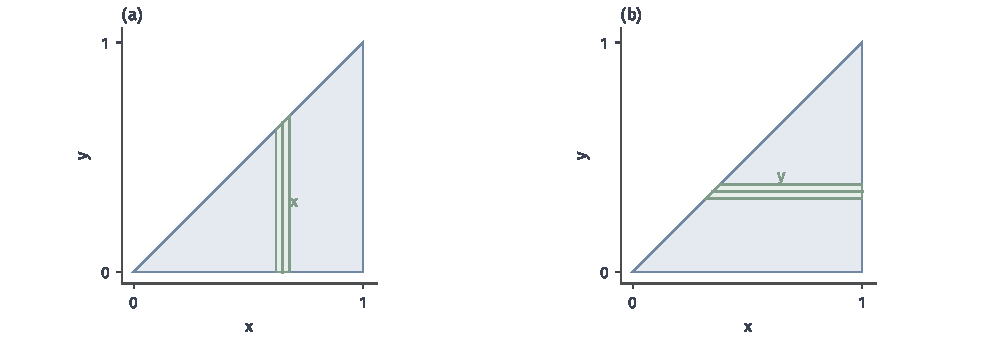
\includegraphics[width=169.0mm]{figures/01-mathematical-preliminaries-upper/00-shared/matplotlib/chapter3-concept-processes/region-slicing-orders.pdf}
 \caption{$D=\{0\leq y\leq x\leq1\}$在两图完全相同。(a) 固定$x$，纵截面为$0\leq y\leq x$；(b) 固定$y$，横截面为$y\leq x\leq1$。绿色窄条仅示意一次切片，图中的条宽不充当实际微元。两种累计$1$都得面积$1/2$；换序依据非负性或绝对可积性，而非图形本身。}
 \label{fig:analysis-process-region-slicing-orders}
\end{figure*}

换序有时决定一个积分能否算出来。
\begin{example}[换序计算含$e^{y^2}$的累次积分]
\label{ex:region-exp-square-order-swap}
考虑
\[
 \int_0^1\left(\int_x^1e^{y^2}\,\mathrm dy\right)\mathrm dx.
\]
内层的$e^{y^2}$没有初等原函数，按原次序无法用原函数直接计算。
积分区域是闭三角形$\{(x,y):0\leq x\leq y\leq1\}$，被积函数在其上连续，因而绝对可积，可以交换次序。
固定$y\in[0,1]$时，横截面是$0\leq x\leq y$，于是
\[
 \int_0^1\left(\int_0^ye^{y^2}\,\mathrm dx\right)\mathrm dy
 =\int_0^1ye^{y^2}\,\mathrm dy
 =\frac{e-1}{2}.
\]
\end{example}

内层对$x$积分时$e^{y^2}$是常数，只产生截面长度$y$，而这个因子$y$恰好使外层积分有原函数$\frac12e^{y^2}$。

\subsubsection{积分换序的适用边界}

非负函数没有正负相消，累计可以为无穷；绝对可积函数允许取正负值，但正负两部分的累计各自有限。
两者都缺失时，两种累计次序可能以不同方式配对正负贡献，交换次序就可能改变结果，甚至一个次序收敛而另一个次序发散。

最直观的例子来自双重级数。
设$a_{i,j}$（$i,j\geq1$）是一个无穷矩阵，在第一象限上令
$f(x,y)=a_{i,j}$于$(x,y)\in[i-1,i)\times[j-1,j)$，即每个边长为$1$的方格上取对应的矩阵元素。
对$x\in[i-1,i)$，截面积分$\int_0^\infty f(x,y)\,\mathrm dy=\sum_ja_{i,j}$是第$i$行的和（在各项非负或该行绝对收敛时）；再对$x$积分，就得到“先行后列”的累次和$\sum_i\sum_ja_{i,j}$。
另一种次序同理给出$\sum_j\sum_ia_{i,j}$，而$\int|f|\,\mathrm dm_2=\sum_{i,j}|a_{i,j}|$。

因此，Tonelli定理说明非负双重级数可以任意交换求和次序，Fubini定理说明绝对收敛的双重级数也可以这样做。
缺少绝对收敛时，即使每一行、每一列的和都有限，两种次序也可能给出不同的结果。

\begin{example}[行列各自可加仍不足以换序]
\label{ex:analysis-iterated-sum-failure}
令$a_{i,j}=\mathbb I\{j=i\}-\mathbb I\{j=i+1\}$（$i,j\geq1$），并按上面的方格构造第一象限上的阶梯函数$f$。
每一行只有一个$1$和一个$-1$，故$\sum_j a_{i,j}=0$；
第一列只有$a_{1,1}=1$，和为$1$；第$j\geq2$列有$a_{j,j}=1$与$a_{j-1,j}=-1$，和为$0$。于是
\[
 \sum_{i=1}^{\infty}\left(\sum_{j=1}^{\infty}a_{i,j}\right)=0,
 \qquad
 \sum_{j=1}^{\infty}\left(\sum_{i=1}^{\infty}a_{i,j}\right)=1,
\]
即$f$的两种累次积分分别为$0$和$1$。
两种累次积分都有有限值，却不相等。每行的绝对值和为$2$，所以$\int|f|\,\mathrm dm_2=+\infty$，
正负部分也各为无穷。失效的是Fubini定理的绝对可积条件，而非某一行的计算规则。
\end{example}

图~\ref{fig:vol1-add-fubini-cancellation-grid}显示这个例子的两条对角线。
逐行求和时，每个$+1$与同一行右侧的$-1$配对；逐列求和时，每个$-1$与同一列下方的$+1$配对，第一列的$+1$则没有配对对象。
由于绝对和无穷，Fubini定理不能保证这两种配对给出同一结果。
\begin{figure}[!htb]
  \centering
  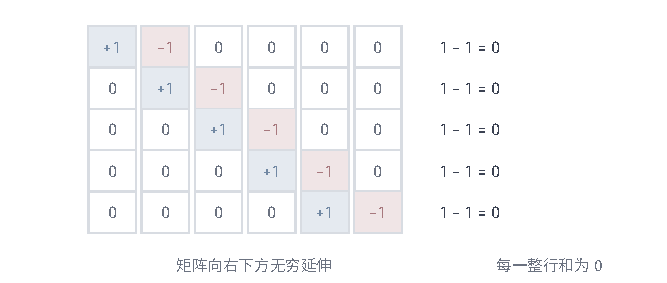
\includegraphics[width=112mm]{figures/01-mathematical-preliminaries-upper/00-shared/tikz/mathematical-language-combinatorics-analysis-optimization-comprehension-additions/fubini-cancellation-grid.pdf}
  \caption{无穷矩阵$a_{i,j}=\mathbb I\{j=i\}-\mathbb I\{j=i+1\}$的左上角，展示前五行、前六列，矩阵向右下方继续；每个单元格也可看成第一象限中边长为$1$的方格。每一整行的和为$0$；第一整列的和为$1$，其他整列的和为$0$。蓝、红单元分别为$+1,-1$，每行绝对和为$2$，因而无穷矩阵不绝对可加。}
  \label{fig:vol1-add-fubini-cancellation-grid}
\end{figure}

连续函数也会出现同样的现象。
\begin{example}[$(x^2-y^2)/(x^2+y^2)^2$的两种累次积分不同]
\label{ex:region-rational-non-fubini}
在$(0,1)^2$上取
\[
 f(x,y)=\frac{x^2-y^2}{(x^2+y^2)^2}.
\]
直接求导可得$\partial_y\bigl(y/(x^2+y^2)\bigr)=f(x,y)$，所以固定$x>0$时
\[
 \int_0^1f(x,y)\,\mathrm dy=\left[\frac{y}{x^2+y^2}\right]_{y=0}^{y=1}=\frac{1}{1+x^2},
\]
再对$x$积分得到$\pi/4$。
由于$f(y,x)=-f(x,y)$，先对$x$积分时内层结果是$-1/(1+y^2)$，这一次序得到$-\pi/4$。

两个结果不同，原因仍是绝对可积性失效。
在$0<y<x$处$f>0$，所以
\[
 \int_0^1|f(x,y)|\,\mathrm dy\geq\int_0^xf(x,y)\,\mathrm dy=\left[\frac{y}{x^2+y^2}\right]_{y=0}^{y=x}=\frac{1}{2x},
\]
而$\int_0^11/(2x)\,\mathrm dx=+\infty$，由Tonelli定理，$\int_{(0,1)^2}|f|\,\mathrm dm_2=+\infty$。
\end{example}

在极坐标下$|f|=|\cos2\theta|/r^2$，这正是示例~\ref{ex:region-power-function-threshold}中$p=2$的临界幂次：原点附近正负两部分各自累计无穷。

\subsection{区域积分的换元}
\label{sec:multivariable-change-variables}

累次积分保留原坐标，只改变累计次序。
换元则用一个向量值映射$T$改变位置的坐标表示，例如用半径与角度描述圆盘中的点。
换坐标以后，函数要按新坐标重写，每个小块的体积也要重新计算：参数空间中大小相同的小块，映到原空间后可能大小不同。

\subsubsection{换元公式与适用条件}

\paragraph{体积的局部缩放}

一元换元$x=T(t)$中，参数的小区间$[t,t+\Delta t]$被映成长约$|T'(t)|\Delta t$的小区间，因子$|T'(t)|$记录长度的缩放（定理~\ref{thm:analysis-lebesgue-change-variables}）。
多元换元要把参数空间中的小块换成体积，先看线性映射。
方阵$\bm A$把单位正方体映成由$\bm A$的各列张成的平行多面体，其体积为$|\det\bm A|$；更一般地，对任意可测集合$E$都有$m_d(\bm AE)=|\det\bm A|\,m_d(E)$\scite{math-folland1999real}。

几个特例可以直接核对。
对角矩阵$\operatorname{diag}(a_1,\ldots,a_d)$分别伸缩各坐标，体积比例为$\prod_j|a_j|$，这正是坐标盒的体积规则。
正交矩阵（旋转与反射）保持距离，不改变图形的形状和大小，行列式为$\pm1$。
剪切矩阵$\begin{bmatrix}1&s\\0&1\end{bmatrix}$把正方形推成等底等高的平行四边形，面积不变，行列式也等于$1$。
公式取行列式的绝对值，是因为反射这类改变定向的映射行列式为负，而体积必须非负。

对可微的非线性映射$T$，由式~\eqref{eq:analysis-jacobian-linearization}，在一点$\bm x$附近有$T(\bm x+\bm h)\approx T(\bm x)+\bm J_T(\bm x)\bm h$。
于是以$\bm x$为角、边长为$\varepsilon$的小方块$Q$，被$T$映成一个近似的平行多面体，其体积约为$|\det\bm J_T(\bm x)|\varepsilon^d$；图~\ref{fig:analysis-process-jacobian-grid-cell}画出了这种小块的变化。

设$g$是原空间中的密度。用小方块$Q_k$铺满参数区域，记$\bm x_k$为$Q_k$的一个角，每块映成的小块$T(Q_k)$中的质量约为
\[
 g(T(\bm x_k))\,m_d(T(Q_k))\approx g(T(\bm x_k))|\det\bm J_T(\bm x_k)|\varepsilon^d.
\]
对$k$求和后，左侧的和近似原空间中的总质量，右侧的和近似参数空间中函数$g(T(\bm x))|\det\bm J_T(\bm x)|$的积分。
因此$g\circ T\,|\det\bm J_T|$是“每单位参数体积所含的质量”：它把原空间中按单位体积计的密度，换算成按参数小块计的密度。

这个局部说明还不是整个积分公式的证明。
整体上还必须控制每块的近似误差在加总以后趋于零，并且确保$T$把每个点只覆盖一次：若两个参数小块映到同一块正体积区域，那里的质量就会被计算两次。

\paragraph{勒贝格积分的换元}

开集之间的$C^1$微分同胚同时满足这两项要求：连续可微保证局部的体积规则，双射保证全局只覆盖一次。
定理直接对勒贝格可测函数陈述，连续被积函数是其特例。
\begin{theorem}[区域积分的换元公式]
设$U,V\subseteq\mathbb R^d$为开集，$T:U\to V$为$C^1$双射，逆映射也为$C^1$，且$\det\bm J_T$处处非零。
对任意非负勒贝格可测函数$g:V\to[0,\infty]$，有
\begin{equation}
 \int_Vg(\bm y)\,\mathrm d\bm y
 =\int_Ug(T(\bm x))|\det\bm J_T(\bm x)|\,\mathrm d\bm x,
 \label{eq:measurable-change-variables}
\end{equation}
允许共同值为$+\infty$。若$g$有符号且在$V$上绝对可积，则变换后的函数也绝对可积，等式仍成立并取有限值。
\end{theorem}

这类变换及其逆在定义域的每个闭有界子集上满足Lipschitz条件，因而把零测集映为零测集。
所以勒贝格可测函数$g$与$T$复合后仍勒贝格可测：Borel集合的原像仍是Borel集合，零测集的原像仍是零测集，而每个勒贝格可测集都是Borel集合与零测集子集之并。

一般定理先建立可测集合的体积变换$m_d(T(E))=\int_E|\det\bm J_T|$，再从指示函数进入简单函数，最后以单调逼近得到非负函数的公式；有符号情形对$|g|$、$g^+$和$g^-$分别应用非负结论即可。
这里说明的是证明的依赖关系，集合层的体积变换定理引用测度论教材\scite{math-folland1999real}，不把逐点线性化当作完整证明。

若只在可测子区域$D\subseteq U$上积分，对$V$中的函数$g\mathbb I_{T(D)}$应用同一公式，即得
\begin{equation}
 \int_{T(D)}g(\bm y)\,\mathrm d\bm y
 =\int_Dg(T(\bm x))|\det\bm J_T(\bm x)|\,\mathrm d\bm x.
 \label{eq:analysis-multivariate-change-variables}
\end{equation}
这里不另加有界或边界零测的要求；所需条件仍是非负可测，或者有符号且绝对可积。

常用坐标在原点、坐标轴或角度的接缝处不是微分同胚，例如极坐标在原点处所有角度都对应同一点。
若在参数区域和原区域中各去掉一个零测集以后，参数化成为开集之间的$C^1$微分同胚，就可以先在剩下的范围内换元，再补回零测集，因为零测集对积分没有贡献。
若参数化在正测度区域上重复覆盖，则不能直接使用这个单次覆盖版本。

\subsubsection{常用坐标变换}

\paragraph{极坐标}

圆盘的边界用直角坐标描述时，积分上下限会含平方根。
以半径$r$和角度$\theta$作为坐标，圆盘变成参数矩形$[0,1]\times[0,2\pi]$，但面积权重必须增加半径因子。
在平面上画出同心圆$r=$常数与射线$\theta=$常数组成的网格：介于$r$与$r+\Delta r$、$\theta$与$\theta+\Delta\theta$之间的小块，径向边长为$\Delta r$，弧向边长约为$r\Delta\theta$，所以面积约为$r\Delta r\Delta\theta$。
同样大小的参数块，离原点越远，对应的面积越大；靠近原点时则被压缩得很小。
这一面积权重正是极坐标映射的Jacobian行列式：示例~\ref{ex:multivariable-polar-jacobian}已算出$\det\bm J=r$。下面用它计算单位圆盘的面积，并检查换元公式的条件。
\begin{example}[用极坐标计算单位圆盘的面积]
\label{ex:analysis-polar-coordinate-jacobian}
令$D=\{\bm x\in\mathbb R^2:\lVert\bm x\rVert_2\leq1\}$，并令$T(r,\theta)=(r\cos\theta,r\sin\theta)$。
在开集$U=(0,1)\times(0,2\pi)$上，$T$是到$V$的$C^1$双射，逆映射也是$C^1$，其中$V$是开圆盘去掉线段$[0,1)\times\{0\}$（含原点）后的区域。
由示例~\ref{ex:multivariable-polar-jacobian}，$|\det\bm J_T(r,\theta)|=r$，在$U$上处处非零。
$D$与$V$只相差边界圆周和线段$[0,1)\times\{0\}$，它们都是零测集，因此
\[
 \int_D1\,\mathrm d\bm x
 =\int_V1\,\mathrm d\bm x
 =\int_0^{2\pi}\int_0^1r\,\mathrm dr\,\mathrm d\theta
 =\pi.
\]
最后一步在参数矩形上使用Tonelli定理，积分上下限包含端点不改变积分值。
若让$\theta$取遍$(0,4\pi)$，圆盘就会被覆盖两次，按公式算出的$2\pi$不再是面积，这正是单次覆盖条件排除的情形。
\end{example}

图~\ref{fig:vol1-add-polar-area-weight}说明半径因子来自哪里。同样的角度变化在较大半径处扫过更长的弧，故同样大小的参数块对应更大的面积，积分权重必须随半径变化。
\begin{figure}[!htb]
  \centering
  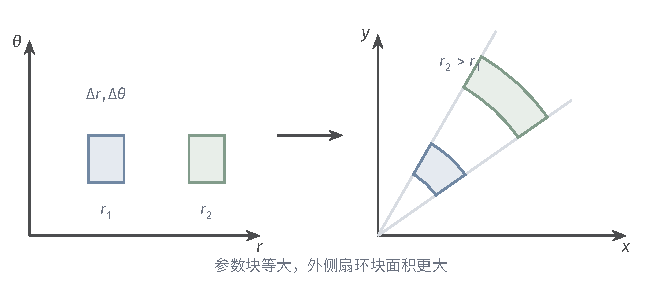
\includegraphics[width=112mm]{figures/01-mathematical-preliminaries-upper/00-shared/tikz/mathematical-language-combinatorics-analysis-optimization-comprehension-additions/polar-area-weight.pdf}
  \caption{极坐标映射中的两个等大参数块，具有相同的$\Delta r,\Delta\theta$，但外侧半径$r_2$较大。对应扇环块的精确面积为$(r\Delta r+(\Delta r)^2/2)\Delta\theta$，一阶项为$r\Delta r\Delta\theta$，因此面积元为$r\,\mathrm dr\,\mathrm d\theta$。图只比较局部块，坐标原点与接缝的处理见正文。}
  \label{fig:vol1-add-polar-area-weight}
\end{figure}

用极坐标可以直接核对示例~\ref{ex:region-power-function-threshold}得到的阈值。
\begin{example}[用极坐标核对幂函数的可积阈值]
\label{ex:region-polar-power-check}
设$0<a<b$，在圆环$\{a\leq\lVert\bm x\rVert_2\leq b\}$上积分$\lVert\bm x\rVert_2^{-p}$。
在开集$(a,b)\times(0,2\pi)$上使用极坐标，被去掉的两条圆周和一条线段都是零测集；被积函数只依赖半径，于是
\[
 \int_{a\leq\lVert\bm x\rVert_2\leq b}\lVert\bm x\rVert_2^{-p}\,\mathrm d\bm x
 =\int_0^{2\pi}\int_a^br^{-p}\cdot r\,\mathrm dr\,\mathrm d\theta
 =2\pi\int_a^br^{1-p}\,\mathrm dr.
\]
令$a\downarrow0$，它有界当且仅当$1-p>-1$，即$p<2$；令$b\to\infty$，它有界当且仅当$1-p<-1$，即$p>2$，与壳层估计一致。
取$p=0$、$a=1$、$b=2$，得到$2\pi\int_1^2r\,\mathrm dr=3\pi$，这就是示例~\ref{ex:region-power-function-threshold}中的$\alpha=m_2(A_0)$。
\end{example}

面积因子$r$正是壳层估计中“面积随半径增长”的来源：半径约为$r$、厚度为$\Delta r$的细圆环，面积约为$2\pi r\Delta r$。

极坐标与累次积分结合，还能计算一个没有初等原函数的一元积分。
\begin{example}[用极坐标计算Gauss积分]
\label{ex:region-gauss-integral}
函数$e^{-x^2}$没有初等原函数，但平面函数$e^{-(x^2+y^2)}$非负，在极坐标下只依赖半径。
对开集$(0,\infty)\times(0,2\pi)$使用换元公式，被去掉的原点和正$x$轴是零测集，于是
\[
 \int_{\mathbb R^2}e^{-(x^2+y^2)}\,\mathrm d(x,y)
 =\int_0^{2\pi}\int_0^\infty e^{-r^2}r\,\mathrm dr\,\mathrm d\theta
 =2\pi\cdot\frac12=\pi.
\]
另一方面，由Tonelli定理，左侧等于
\[
 \begin{aligned}
 \int_{\mathbb R}\left(\int_{\mathbb R}e^{-x^2}e^{-y^2}\,\mathrm dy\right)\mathrm dx
 &=\int_{\mathbb R}e^{-x^2}\,\mathrm dx\cdot\int_{\mathbb R}e^{-y^2}\,\mathrm dy\\
 &=\left(\int_{\mathbb R}e^{-x^2}\,\mathrm dx\right)^2.
 \end{aligned}
\]
这个积分为正，因此$\int_{\mathbb R}e^{-x^2}\,\mathrm dx=\sqrt\pi$。
\end{example}

这个结果给出正态分布密度的归一化常数。
计算同时用到了换元和累次积分：换元把平面积分变成可算的径向积分，累次积分把同一个平面积分拆成两个相同的一元积分。

\paragraph{柱坐标}

在三维中，柱坐标在极坐标之外保留高度$z$：
\[
 (x,y,z)=(r\cos\theta,r\sin\theta,z).
\]
参数小块对应的是一块极坐标小块再沿竖直方向拉高$\Delta z$，体积约为$r\Delta r\Delta\theta\Delta z$。
Jacobian矩阵左上角是极坐标的$2\times2$块，右下角为$1$，其余元素为零，行列式仍为$r$，故体积元是$r\,\mathrm dr\,\mathrm d\theta\,\mathrm dz$。
用这个体积元可以直接算出圆柱体的体积。
\begin{example}[圆柱体的体积]
\label{ex:region-cylinder-volume}
半径$R$、高度$H$的圆柱体由$0\leq r\leq R$、$0\leq\theta\leq2\pi$、$0\leq z\leq H$描述。
与极坐标相同，在开参数长方体$(0,R)\times(0,2\pi)\times(0,H)$上换元，去掉的竖直半平面片和圆柱表面都是零测集。于是
\[
 \int_0^H\int_0^{2\pi}\int_0^R r\,\mathrm dr\,\mathrm d\theta\,\mathrm dz
 =H\cdot2\pi\cdot\frac{R^2}{2}=\pi R^2H.
\]
\end{example}

关于竖直轴对称的物体，如圆柱、圆锥、旋转抛物面所围的区域，用柱坐标描述时上下限最简单。

\paragraph{球坐标}

球坐标用到原点的距离$\rho$、从正$z$轴量起的夹角$\varphi$和绕$z$轴的角$\theta$：
\[
 (x,y,z)=(\rho\sin\varphi\cos\theta,\rho\sin\varphi\sin\theta,\rho\cos\varphi).
\]
在球面上，$\varphi$相当于纬度（从北极量起），$\theta$相当于经度。
参数小块对应的近似长方体有三条边：沿径向长$\Delta\rho$；沿经线长$\rho\Delta\varphi$；沿纬线圆长$\rho\sin\varphi\Delta\theta$，因为纬线圆的半径是$\rho\sin\varphi$。
三边相乘得到体积约为$\rho^2\sin\varphi\,\Delta\rho\Delta\varphi\Delta\theta$；靠近两极时纬线圆变小，参数小块对应的体积也随之变小。

按$(\rho,\varphi,\theta)$的次序写出Jacobian矩阵，沿第三行展开行列式，
\[
 \det\begin{bmatrix}
 \sin\varphi\cos\theta&\rho\cos\varphi\cos\theta&-\rho\sin\varphi\sin\theta\\
 \sin\varphi\sin\theta&\rho\cos\varphi\sin\theta&\rho\sin\varphi\cos\theta\\
 \cos\varphi&-\rho\sin\varphi&0
 \end{bmatrix}
\]
等于
\[
 \cos\varphi\cdot\rho^2\sin\varphi\cos\varphi+\rho\sin\varphi\cdot\rho\sin^2\varphi
 =\rho^2\sin\varphi,
\]
与几何估计一致；在$0<\varphi<\pi$上它为正，故体积元为$\rho^2\sin\varphi\,\mathrm d\rho\,\mathrm d\varphi\,\mathrm d\theta$。
用这个体积元可以算出球的体积。
\begin{example}[球的体积]
\label{ex:region-ball-volume}
半径$R$的球由$0\leq\rho\leq R$、$0\leq\varphi\leq\pi$、$0\leq\theta\leq2\pi$描述。
和极坐标一样，在开参数长方体$(0,R)\times(0,\pi)\times(0,2\pi)$上换元，它覆盖的是球内部去掉半平面片$\{y=0,\ x\geq0\}$后的区域；被去掉的半平面片（其中包含$z$轴上的一段）与球面都是零测集，补回后不改变积分。于是
\[
 \int_0^{2\pi}\int_0^\pi\int_0^R\rho^2\sin\varphi\,\mathrm d\rho\,\mathrm d\varphi\,\mathrm d\theta
 =2\pi\cdot2\cdot\frac{R^3}{3}
 =\frac{4\pi R^3}{3},
\]
其中$\int_0^\pi\sin\varphi\,\mathrm d\varphi=2$，$\int_0^R\rho^2\,\mathrm d\rho=R^3/3$。
\end{example}

球在球坐标下变成参数长方体，三组上下限都是常数；以原点为中心对称的区域，或只依赖$\rho$的被积函数，用球坐标计算最简单。

\subsection{参数积分}
\label{sec:multivariable-parameter-integrals}

换元改变的是空间坐标。
参数积分则固定积分区域，让被积函数依赖一个实参数$\theta$，研究积分所得的总量怎样随参数变化。
例如$\theta$是时间，$g(\bm x,\theta)$是时刻$\theta$的质量密度，积分就是该时刻的总质量；或者$\theta$是模型中的参数，积分是依赖该参数的平均损失。
这里要回答三个问题：总量是否随参数连续变化，总量的变化率能否由密度的变化率累计得到，以及积分区间的端点也随参数移动时怎样求导。

\subsubsection{参数积分的定义}

设$D\in\mathcal L(\mathbb R^d)$，$I$为实参数区间，且对每个$\theta\in I$，$g(\cdot,\theta)$都是$D$上可积的标量函数。定义
\[
 G(\theta)=\int_Dg(\bm x,\theta)\,\mathrm d\bm x.
\]
固定参数后，$\bm x$是被积变量；积分完成以后，$G$是参数$\theta$的一元函数。
例如$D=[0,\infty)$、$g(x,\theta)=e^{-\theta x}$（$\theta>0$）时，$G(\theta)=1/\theta$。

点态连续或点态可微只描述每个固定位置$\bm x$处的变化。
总量$G$还可能因为“质量”在参数变化时移向无穷远，或集中到越来越小的区域而突变，这些现象在任何固定位置都看不出来。
下面的例子中，密度在每一点都趋于零，总质量却保持不变。
\begin{example}[$\theta e^{-\theta x}$的质量逃向无穷远]
\label{ex:region-escaping-mass}
在$[0,\infty)$上令$g(x,\theta)=\theta e^{-\theta x}$（$\theta>0$）。对每个$\theta>0$，
\[
 G(\theta)=\int_0^\infty\theta e^{-\theta x}\,\mathrm dx=1.
\]
另一方面，$\theta\downarrow0$时，对每个固定的$x$都有$g(x,\theta)\to0$。
质量被摊薄并推向远处：由$\int_c^\infty\theta e^{-\theta x}\,\mathrm dx=e^{-\theta c}$，总质量的一半位于$x\geq(\log2)/\theta$的位置，而这个位置随$\theta\downarrow0$趋于无穷远。
若在$\theta=0$处按点态极限令$g(x,0)=0$，则$G(0)=0\neq1=\lim_{\theta\downarrow0}G(\theta)$。
\end{example}

可见点态极限本身不能决定总量的极限；要把点态性质传递给$G$，还需要控制整族函数，防止质量逃逸。

\subsubsection{参数积分的连续性}

所需的控制由支配收敛定理提供：用同一个可积函数控制附近全部参数的密度，贡献就不能集中到越来越小的区域，也不能移向无穷远。
\begin{theorem}[可积控制下参数积分的连续性]
设$\theta_0\in I$，每个$g(\cdot,\theta)$可测。假设存在$\theta_0$在$I$中的一个相对邻域$J$、同一个可测零测集$N$及非负可积函数$h$，使对每个$\bm x\in D\setminus N$，$g(\bm x,\cdot)$在$\theta_0$连续，且
$|g(\bm x,\theta)|\leq h(\bm x)$对所有$\theta\in J$成立。
则$G(\theta)$在$J$上有有限值，并在$\theta_0$连续。
\end{theorem}
\begin{proof}
任取$\theta_n\to\theta_0$，充分大时$\theta_n\in J$。在$D\setminus N$上，$g(\bm x,\theta_n)\to g(\bm x,\theta_0)$，且绝对值都不超过$h(\bm x)$。
支配收敛给出$G(\theta_n)\to G(\theta_0)$，由序列判据得到连续性。
\end{proof}

控制函数$h$的作用是给所有邻近参数的密度一个共同的、总量有限的上方包络，质量就无法逃到包络以外。
示例~\ref{ex:region-escaping-mass}中不存在这样的包络：对任意$\delta>0$，当$x>1/\delta$时，
\[
 \sup_{0<\theta<\delta}\theta e^{-\theta x}=\frac{1}{ex},
\]
上确界在$\theta=1/x$处取到，而$1/(ex)$在$(1/\delta,\infty)$上不可积。

相反，对$g(x,\theta)=e^{-\theta x}$，固定$\theta_0>0$，在邻域$\theta>\theta_0/2$内有$e^{-\theta x}\leq e^{-\theta_0x/2}$，后者在$[0,\infty)$上可积，故$G$在$\theta_0$连续。
控制函数只需覆盖所考察参数点的邻域，不要求同一上界适用于全部参数；这里每个$\theta_0>0$各用一个包络，就得到$G$在整个$(0,\infty)$上连续。

\subsubsection{积分号下求导}

若$g(\bm x,\theta)$是时刻$\theta$的密度，自然希望总质量的变化率等于各处密度变化率的累计，即$G'(\theta)=\int_D\partial_\theta g(\bm x,\theta)\,\mathrm d\bm x$。
这实际是交换参数差商的极限与积分。
各点偏导数存在只确定差商的点态极限；用同一个可积函数控制全部差商，才足以将这个极限移入积分号。
\begin{theorem}[可积导数界下的积分号内求导]
设$I$是包含$\theta_0$的开区间，对每个$\theta\in I$，$\bm x\mapsto g(\bm x,\theta)$可测，并且$g(\cdot,\theta_0)$可积。
假设存在一个可测零测集$N$，使每个$\bm x\in D\setminus N$处的$\theta\mapsto g(\bm x,\theta)$在整个$I$内可微；对每个$\theta$，偏导数作为$\bm x$的函数可测，并且存在非负可积函数$h$使
\begin{equation}
 \left|\frac{\partial g}{\partial\theta}(\bm x,\theta)\right|\leq h(\bm x)
 \quad\text{对所有$\bm x\in D\setminus N$及所有$\theta\in I$成立},
 \label{eq:analysis-parameter-derivative-domination}
\end{equation}
则对每个$\theta\in I$，$g(\cdot,\theta)$在$D$上可积，且
\begin{equation}
 G'(\theta_0)=\int_D\frac{\partial g}{\partial\theta}(\bm x,\theta_0)\,\mathrm d\bm x.
 \label{eq:analysis-differentiate-under-integral}
\end{equation}
\end{theorem}
\begin{proof}
对$\bm x\notin N$，一元中值定理给出
$|g(\bm x,\theta)-g(\bm x,\theta_0)|\leq|\theta-\theta_0|h(\bm x)$，
所以$I$中每个$g(\cdot,\theta)$都被可积函数$|g(\cdot,\theta_0)|+|\theta-\theta_0|h$控制，因而可积，$G$在$I$内有有限值。
对非零$t$且$\theta_0+t\in I$，令
\[
 q_t(\bm x)=\frac{g(\bm x,\theta_0+t)-g(\bm x,\theta_0)}{t}.
\]
中值定理又给出
\[
 |q_t(\bm x)|\leq h(\bm x)\qquad(\bm x\notin N),
\]
并且$t\to0$时，$q_t(\bm x)$在$D\setminus N$上趋于$\partial g/\partial\theta(\bm x,\theta_0)$。
对任意非零序列$t_n\to0$应用支配收敛，都得到同一个积分极限$\int_D\partial_\theta g(\bm x,\theta_0)\,\mathrm d\bm x$；
由实数极限的序列判据，它就是差商$\bigl(G(\theta_0+t)-G(\theta_0)\bigr)/t$在$t\to0$时的极限，即式~\eqref{eq:analysis-differentiate-under-integral}。
\end{proof}

这里的零测集$N$和控制函数$h$都不能随参数改变：参数范围不可数，不能靠取全部参数例外集的并自动获得一个零测集。
条件~\eqref{eq:analysis-parameter-derivative-domination}是一组便于核对的充分条件；更一般的版本也可以直接控制参数差商。

控制函数通常只在所考察参数点的一个邻域内取得。
\begin{example}[对$e^{-\theta x}$在积分号下求导]
\label{ex:region-differentiate-exponential}
令$g(x,\theta)=e^{-\theta x}$，$x\in[0,\infty)$、$\theta>0$，则$G(\theta)=1/\theta$。
固定$\theta_0>0$，取$I=(\theta_0/2,3\theta_0/2)$，则对$\theta\in I$，
\[
 |\partial_\theta g(x,\theta)|=xe^{-\theta x}\leq xe^{-\theta_0x/2}=:h(x).
\]
分部积分给出$\int_0^\infty h(x)\,\mathrm dx=4/\theta_0^2<\infty$；不等式对每个$x$都成立，可取$N=\varnothing$。
由积分号下求导的定理，
\[
 G'(\theta_0)=-\int_0^\infty xe^{-\theta_0x}\,\mathrm dx=-\frac{1}{\theta_0^2},
\]
与$G(\theta)=1/\theta$的直接求导一致。
\end{example}

例中的控制函数依赖于$\theta_0$：若参数范围包含任意接近零的正数，$xe^{-\theta_0x/2}$就不再控制全部导数。
交换求导与积分所需的，只是所考察参数点附近的统一控制。

若所考察参数点附近找不到可积的导数界，交换求导与积分可能失败。
下面的反例发生在参数区间的端点$\theta=0$，考察的是右导数。
\begin{example}[参数积分中的控制函数失效]
\label{ex:analysis-parameter-integral-failure}
对$\theta\geq0$与$x\in(0,1)$，定义
\[
 g(x,\theta)=
 \begin{cases}
 \dfrac{\theta x}{x^2+\theta^2}, & \theta>0,\\[5pt]
 0, & \theta=0.
 \end{cases}
\]
在$\theta=0$处，对每个固定$x>0$，差商$g(x,\theta)/\theta=x/(x^2+\theta^2)\to1/x$，所以关于$\theta$的右偏导数都等于$1/x$，但$1/x$在$(0,1)$上不可积。
直接积分（令$u=x^2+\theta^2$）得到
\[
 G(\theta)=\frac{\theta}{2}\log\left(\frac{1+\theta^2}{\theta^2}\right)\quad(\theta>0),
 \qquad G(0)=0.
\]
于是$G(\theta)/\theta=\frac12\log(1+\theta^{-2})$在$\theta\downarrow0$时发散，$G$在$0$处没有有限右导数。
积分内的逐点右导数虽然存在，却缺少统一可积控制，因此这里不能交换右求导与积分。
\end{example}

从密度的角度看，$g(\cdot,\theta)$在$x=\theta$处取峰值$1/2$；$\theta$变小时峰值向原点移动，差商$g(\cdot,\theta)/\theta$在峰值处等于$1/(2\theta)$，它的累计随之变得无界。

\subsubsection{变限积分的求导}

积分号下求导的定理固定了积分区域。
端点也变化时，即使被积函数不依赖参数，积分仍然会变化：例如$G(\theta)=\int_0^\theta1\,\mathrm dx=\theta$的导数为$1$，而被积函数对参数的偏导数为零，只累计偏导数会遗漏端点移动的贡献。

用质量来理解：区间$[a(\theta),b(\theta)]$上的总质量有两种变化来源，一是区间内部各处的密度在变，二是端点移动时把新的位置划入或划出区间。
右端点在参数增加$\Delta\theta$时向右移动约$b'(\theta)\Delta\theta$，新划入的一小段上密度约为$g(b(\theta),\theta)$，带来质量约$g(b(\theta),\theta)b'(\theta)\Delta\theta$；左端点向右移动则划出一小段，减少质量约$g(a(\theta),\theta)a'(\theta)\Delta\theta$。
要用端点处的函数值估计这一小段的质量，被积函数需要在端点附近连续。
\begin{theorem}[变限参数积分的求导]
设$a(\theta),b(\theta)$在$\theta_0$附近可微，且$a(\theta)<b(\theta)$。
若$g(x,\theta)$和$\partial_\theta g(x,\theta)$在包含这些邻近积分区间的一个紧矩形上连续，则
\begin{equation}
 \begin{aligned}
 \frac{\mathrm d}{\mathrm d\theta}\int_{a(\theta)}^{b(\theta)}g(x,\theta)\,\mathrm dx
 &=\int_{a(\theta)}^{b(\theta)}\partial_\theta g(x,\theta)\,\mathrm dx\\
 &\quad+g(b(\theta),\theta)b'(\theta)
 -g(a(\theta),\theta)a'(\theta).
 \end{aligned}
\label{eq:measurable-moving-boundary-integral}
\end{equation}
\end{theorem}
\begin{proof}
记$a_0=a(\theta_0)$、$b_0=b(\theta_0)$。积分差可分解为
\[
 \begin{aligned}
 G(\theta)-G(\theta_0)
 &=\int_{a_0}^{b_0}\bigl[g(x,\theta)-g(x,\theta_0)\bigr]\,\mathrm dx\\
 &\quad+\int_{b_0}^{b(\theta)}g(x,\theta)\,\mathrm dx
 -\int_{a_0}^{a(\theta)}g(x,\theta)\,\mathrm dx.
 \end{aligned}
\]
短区间积分按端点次序采用有向约定。
第一项是固定区间上的参数积分：$\partial_\theta g$在紧矩形上连续，因而有界，常数界在有界区间$[a_0,b_0]$上可积，满足条件~\eqref{eq:analysis-parameter-derivative-domination}，所以第一项除以$\theta-\theta_0$后趋于$\int_{a_0}^{b_0}\partial_\theta g(x,\theta_0)\,\mathrm dx$。
$g$在紧矩形上一致连续，当$\theta\to\theta_0$时，短区间$[b_0,b(\theta)]$上的$g(x,\theta)$一致地接近$g(b_0,\theta_0)$，所以第二项等于
$g(b_0,\theta_0)[b(\theta)-b_0]+o(|b(\theta)-b_0|)$。端点的可微性保证$|b(\theta)-b_0|=O(|\theta-\theta_0|)$，所以它的差商趋于$g(b_0,\theta_0)b'(\theta_0)$。
第三项同理，并保留前面的负号，得到下端点贡献。三项相加即得公式。
\end{proof}

紧矩形上的连续性是一组便于核对的充分条件。
对一般可测函数，公式中的端点值$g(b(\theta),\theta)$需要另外赋予意义：几乎处处相等的两个函数可以在端点上取不同的值，不能从几乎处处的等价类中直接读出边界上的值。

\FloatBarrier
